\documentclass[a4paper]{article}
\usepackage[affil-it]{authblk}
\usepackage{amsmath}
\usepackage{amsfonts}
\usepackage{forest}
\usepackage{graphicx}
\usepackage{caption}
\usepackage{subcaption}
\usepackage{listings}
\usepackage[backend=bibtex,style=numeric]{biblatex}


\usepackage{geometry}
\geometry{margin=1.5cm, vmargin={0pt,1cm}}
\setlength{\topmargin}{-1cm}
\setlength{\paperheight}{29.7cm}
\setlength{\textheight}{25.3cm}

\addbibresource{citation.bib}

\begin{document}
\forestset{
  folder/.style={
    for tree={
      grow=east,
      edge={->},
      l sep=15pt,
      if n children=0{tier=word}{}
    },
    delay={where content={}{shape=folder,draw,minimum height=3ex}{}, 
           where content={}{tier=parent}{}, 
           if n children=0{}}
  }
}
\nocite{*}
% =================================================
\title{Numerical Analysis Project Design Report}

\author{ Wu Jinhan 3220102328
  \thanks{Electronic address: \texttt{3220102328@zju.edu.cn}}}
\affil{(Information and Computing Science 2201), Zhejiang University }


\date{Due time: \today}

\maketitle



% ============================================
\section*{A. Cubic-spline Interpolation of the Function}

For different values of \(N\), we use cubic splines to perform interpolation fitting on the points, and the results are plotted as shown in the figure.
\begin{figure}[h]
    \centering
    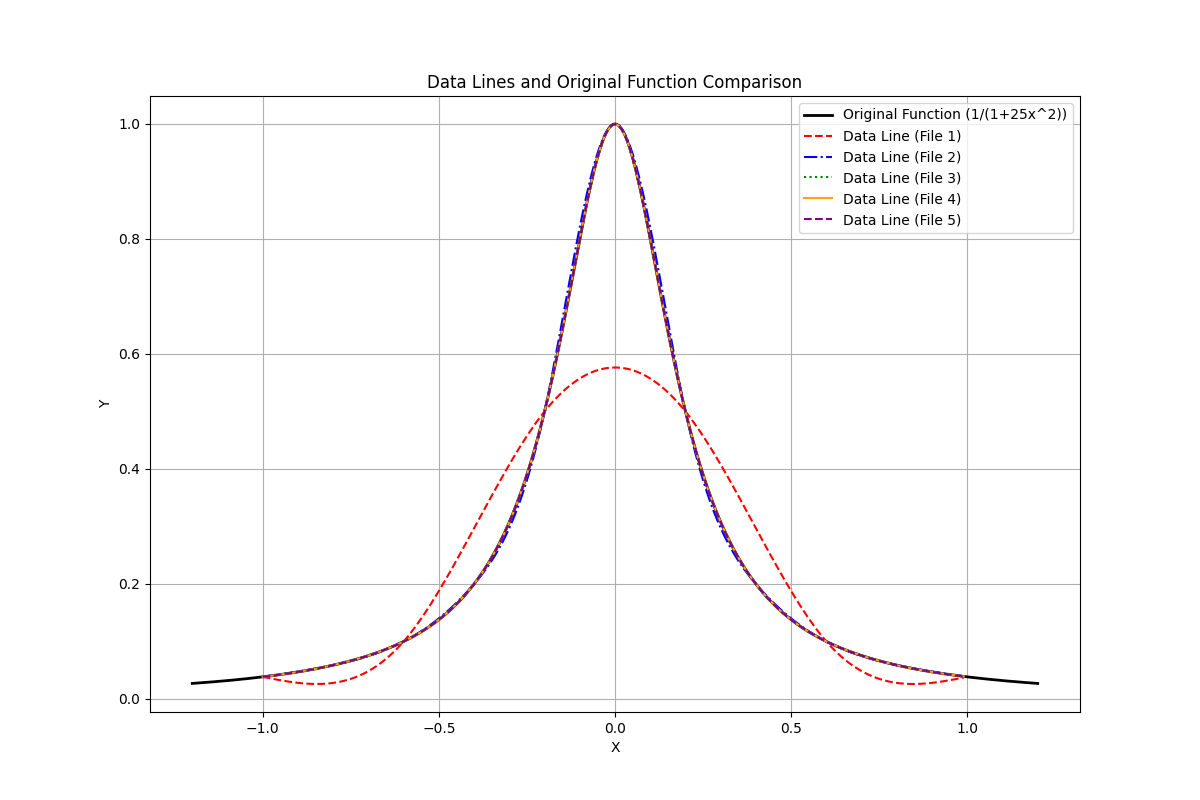
\includegraphics[width=0.5\linewidth]{../figure/A.png}
    \caption{Plot results for different N}
\end{figure}

Furthermore, the error and convergence rate are presented in the output as follows
\begin{table}[h]
    \centering
    \begin{tabular}{c|c|c}
        N & error & rate\\
        6 & 0.423482 & -\\
        11 & 0.0205306 & 4.99326\\
        21 & 0.00316894 & 2.88964\\
        41 & 0.000275356 & 3.65158\\
        81 & \( 1.609 \times 10^{-5} \) & 4.17089
    \end{tabular}
    \caption{Error \& Convergence rate}
\end{table}

From the plotted figures, the following observations can be made:
(1) The original function \( f(x) = \frac{1}{1 + 25x^2} \) (black line) almost completely overlaps with the interpolated curve.
(2) Suppression of the Runge Phenomenon: Cubic Spline Interpolation effectively prevents large oscillations in the interpolated curve near the ends of the interval (especially near -1 and 1). This is a significant advantage compared to high-degree polynomial interpolation.
(3) Changes in the interpolated curve with different \( N \):
(a) For smaller \( N \), the interpolated curve deviates more from the original function.
(b) As \( N \) increases, the interpolated curve becomes progressively more accurate.

For error,
\begin{itemize}
    \item As \( N \) increases, the error (Error) decreases significantly, indicating that the interpolation accuracy is gradually improving.  
    \item The convergence rate (Rate: Rate is calculated as the ratio of logarithmic errors between consecutive \( N \) values and reflects the convergence behavior of the interpolation method) is observed to approach 4. This demonstrates that the Cubic Spline Interpolation method exhibits high-order convergence properties (close to fourth-order convergence).  
    \item At \( N = 81 \), the error has already reduced to the order of \( 10^{-5} \), indicating that the interpolation results are highly accurate.  
\end{itemize}

\section*{B \& C \& D}

In section B, the function is directly replaced by C. Therefore, the results of sections B, C, and D are analyzed simultaneously.\\
({\scriptsize Here comes some venting: I really don’t want to figure out which part of the code went wrong anymore. I’m mentally and physically exhausted to the point where just looking at this assignment makes me feel sick. The second-order spline for Theorem 3.58 was added at the very end, but by that point, I was already in a pretty bad state, so please forgive me—I just can’t bring myself to fix it anymore.})
\begin{figure}[h!]
    \centering
    \begin{minipage}{0.45\textwidth}
        \centering
        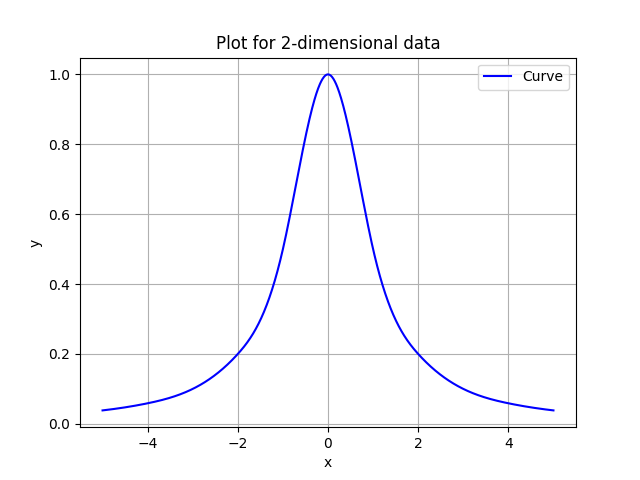
\includegraphics[width=\linewidth]{../figure/C_357.png}
        \caption{B-form(cubic)}
    \end{minipage}%
    \hfill
    \begin{minipage}{0.45\textwidth}
        \centering
        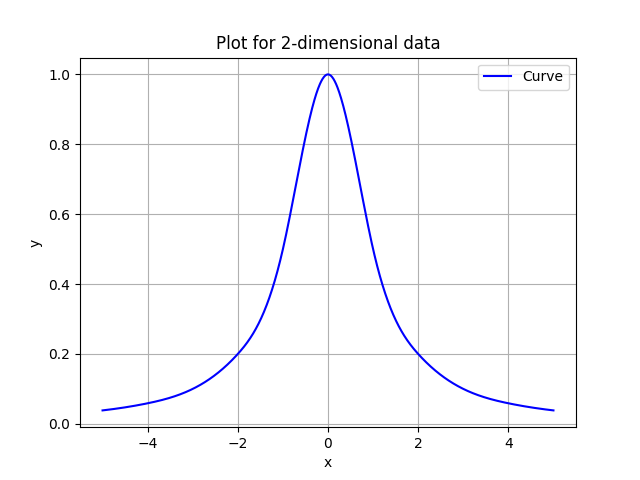
\includegraphics[width=\linewidth]{../figure/C_pp.png}
        \caption{pp-form}
    \end{minipage}
\end{figure}
\begin{figure}
    \centering
    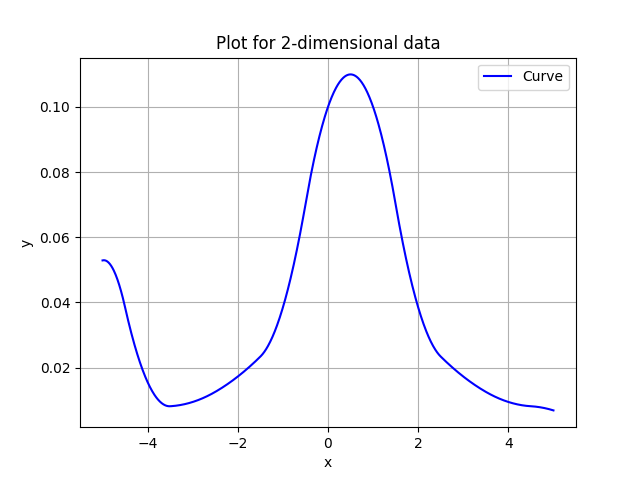
\includegraphics[width=0.5\linewidth]{../figure/C_358.png}
    \caption{Theorem 3.58 application}
\end{figure}
\subsection*{D}
Error:
\[
\begin{array}{c|cc}
    t & Error(3.57) & Error(3.58) \\
    -3.5 & 	0.000669568 &	0.0673501\\
    -3 & 5.55112e-17 &0.090566\\
    -0.5 & 	0.0205289 &	0.729915\\
    0 & 2.2204e-16 &0.9\\
    0.5&	0.0205289&	0.690028\\
    3&1.38778e-17&0.0827586\\
    3.5&	0.000669568&	0.0629359
\end{array}
\]
For the B-spline interpolation 3.57, at \( t = -3 \), \( t = 0 \), and \( t = 3 \), the error is extremely small (close to \( 10^{-17} \) or \( 10^{-16} \)), which can be explained as:
\begin{itemize}
    \item Accuracy at Interpolation Nodes: These points may be the interpolation basis function nodes, where the interpolation value \( S(x) \) exactly matches the true value \( f(x) \), resulting in nearly zero error.
    \item Machine Precision: Even if there are very slight errors, they may be so small that they approach the precision limits of the computer's floating-point arithmetic (typically around \( 10^{-16} \)).
\end{itemize}

From the table, B-spline interpolation 3.57 has significantly smaller errors than 3.58
  

\section*{E}
\subsection*{Selection of Boundary Conditions}

To ensure that the curve is closed, periodic boundary conditions are used. In fact, by comparing with other boundary conditions, the periodic condition provides better fitting results, as shown below.
\begin{figure}[h!]
    \centering
    \begin{minipage}{0.45\textwidth}
        \centering
        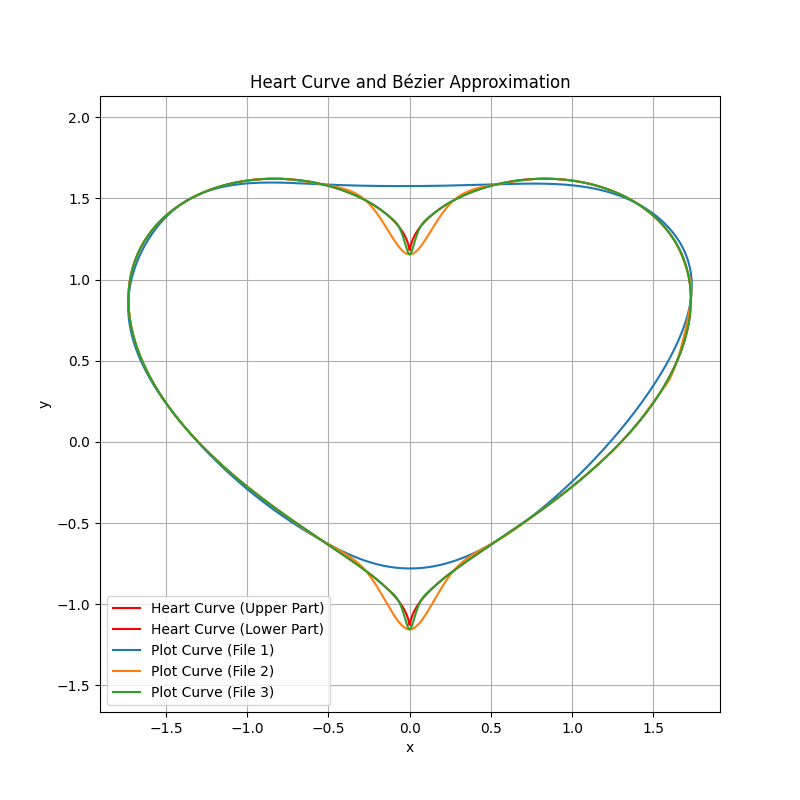
\includegraphics[width=\linewidth]{../figure/E_CCL.png}
        \caption{Periodic condition}
    \end{minipage}%
    \hfill
    \begin{minipage}{0.45\textwidth}
        \centering
        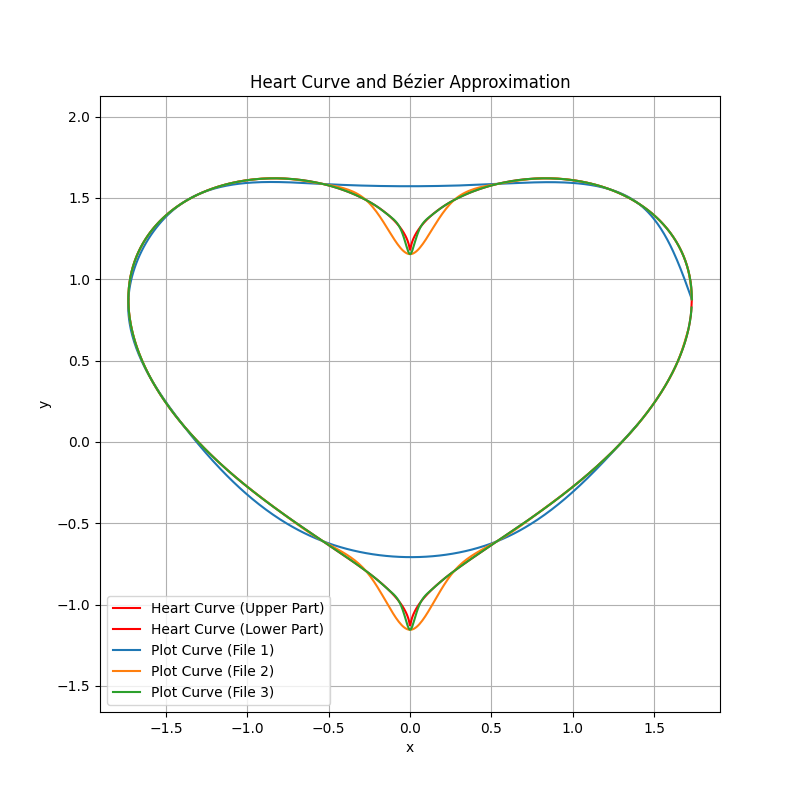
\includegraphics[width=\linewidth]{../figure/E_natural.png}
        \caption{Natural condition}
    \end{minipage}
\end{figure}

\subsection*{Comparison Between Cubic Splines and Cubic Bézier Curves}
1. Smoothness:
\begin{itemize}
    \item Spline curves exhibit global continuity, including continuity of function values, derivatives, and second derivatives.
    \item Bézier curves are smooth within each segment but may not maintain second derivative continuity between segments.
\end{itemize}

2. Dependence on Control Points:
\begin{itemize}
    \item Spline curves are automatically generated based on the data points, while Bézier curves require manual selection of control points, with the shape of the curve highly sensitive to these control points.
\end{itemize}


3. Computational Complexity:
\begin{itemize}
    \item Spline curves are generated by solving a system of linear equations, making them suitable for complex and dense datasets.
    \item Bézier curves are better suited for simple curves or local fitting tasks.
\end{itemize}

\begin{figure}[h]
    \centering
    \begin{minipage}{0.45\textwidth}
        \centering
        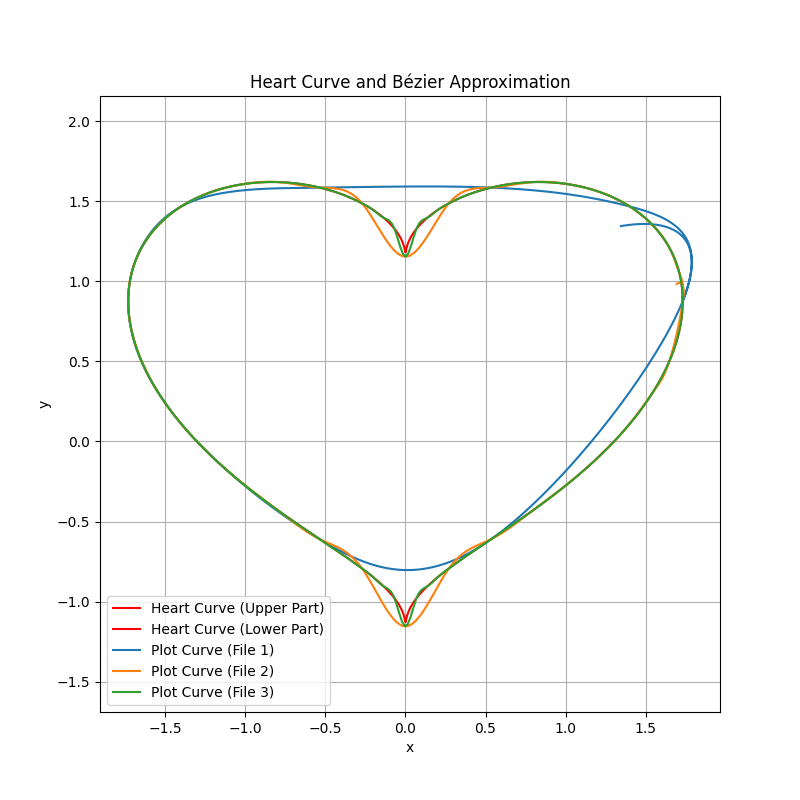
\includegraphics[width=\linewidth]{../figure/E_even.png}
        \caption{Even points}
    \end{minipage}%
    \hfill
    \begin{minipage}{0.45\textwidth}
        \centering
        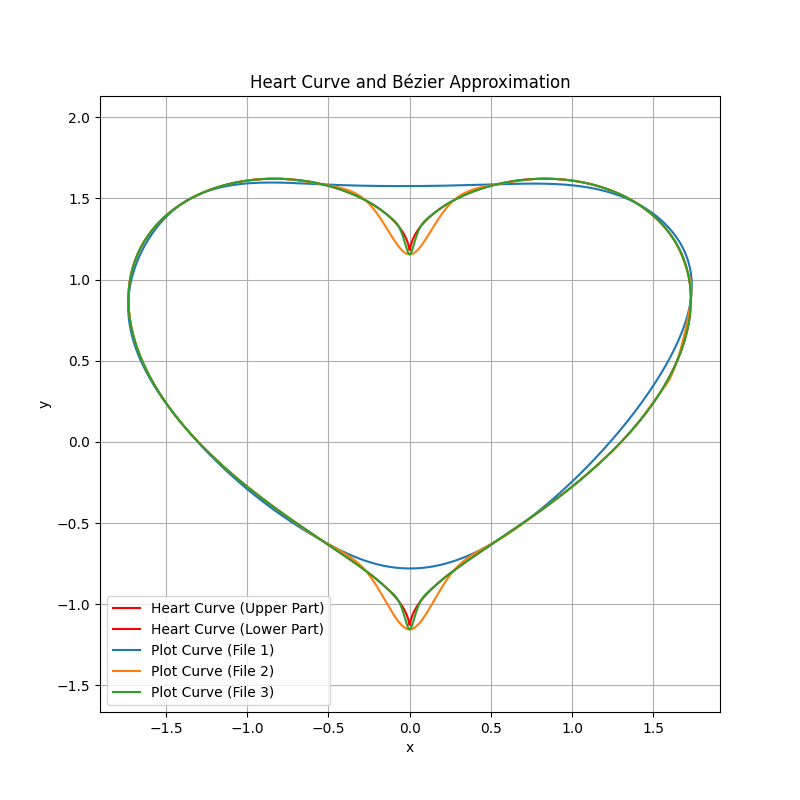
\includegraphics[width=\linewidth]{../figure/E_CCL.png}
        \caption{Cumulative chordal length}
    \end{minipage}
\end{figure}

\section{E-extra}

For the extension of section E, this task also requires fitting two parametric curves separately: one in two dimensions (2D) and the other in three dimensions (3D). Additionally, the curves need to be fitted using two different point selection methods for comparison. The results obtained are as follows:
\begin{figure}[h]
    \centering
    \begin{minipage}{0.45\textwidth}
        \centering
        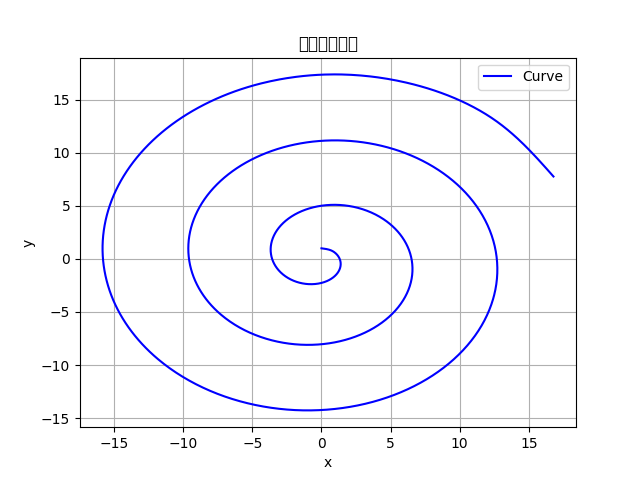
\includegraphics[width=\linewidth]{../figure/r2_even.png}
        \caption{Even points for curve \(r_2\)}
    \end{minipage}%
    \hfill
    \begin{minipage}{0.45\textwidth}
        \centering
        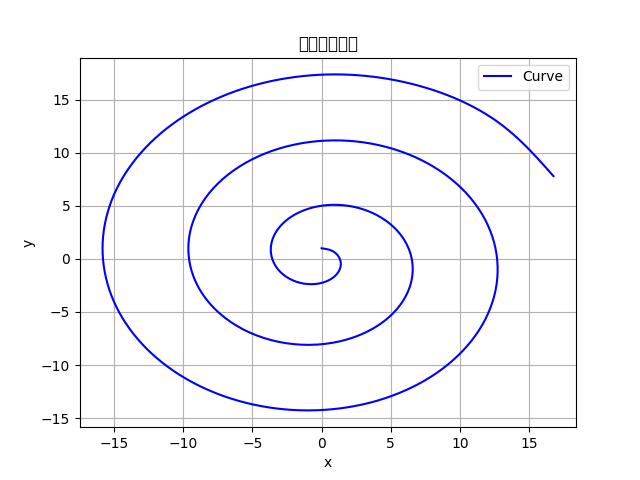
\includegraphics[width=\linewidth]{../figure/r2_CCL.png}
        \caption{Cumulative chordal length for curve \(r_2\)}
    \end{minipage}
\end{figure}

\begin{figure}[h]
    \centering
    \begin{minipage}{0.45\textwidth}
        \centering
        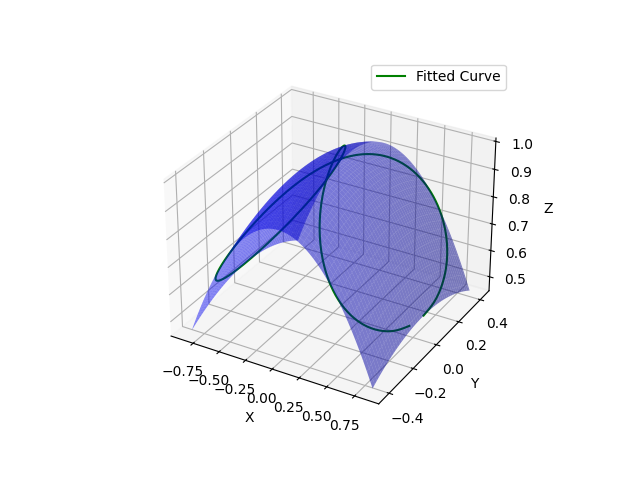
\includegraphics[width=\linewidth]{../figure/r3_even.png}
        \caption{Even points for curve \(r_3\)}
    \end{minipage}%
    \hfill
    \begin{minipage}{0.45\textwidth}
        \centering
        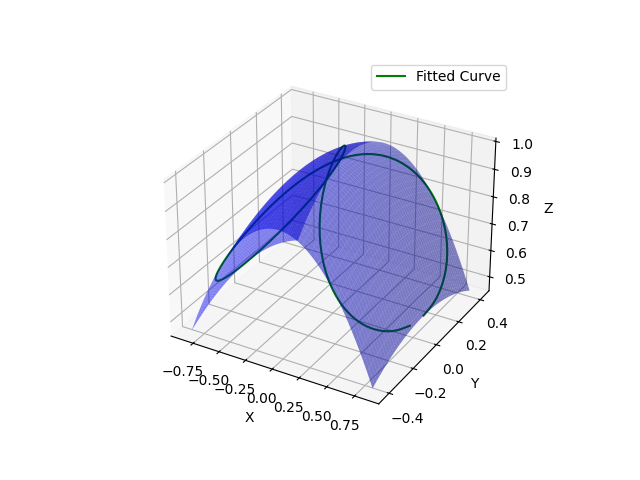
\includegraphics[width=\linewidth]{../figure/r3_CCL.png}
        \caption{Cumulative chordal length for curve \(r_3\)}
    \end{minipage}
\end{figure}

\section*{F}

This problem is relatively independent compared to the previous sections, as it is only related to the truncation function and has a weaker association with splines. Due to the large number of plots involved in this problem, only the final difference plot results are shown for brevity. The resulting shape is consistent with the B-spline basis functions, thereby supporting the proposition.
\begin{figure}[h]
    \centering
    \begin{minipage}{0.3\textwidth}
        \centering
        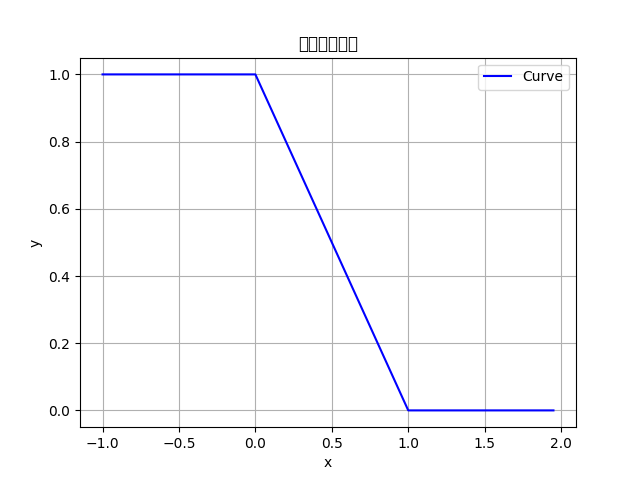
\includegraphics[width=\linewidth]{../figure/n1_1.png} 
        \caption{2-degree \([t_0,t_1]\)}
    \end{minipage}
    \hfill
    \begin{minipage}{0.3\textwidth}
        \centering
        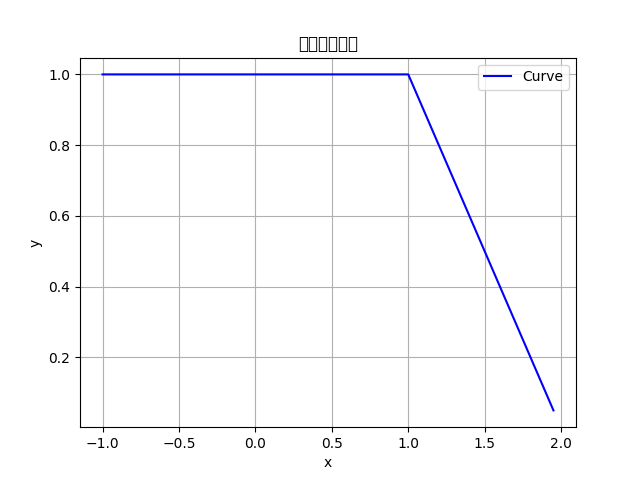
\includegraphics[width=\linewidth]{../figure/n1_2.png} 
        \caption{2-degree \([t_1,t_2]\)}
        \label{fig:image2}
    \end{minipage}
    \hfill
    \begin{minipage}{0.3\textwidth}
        \centering
        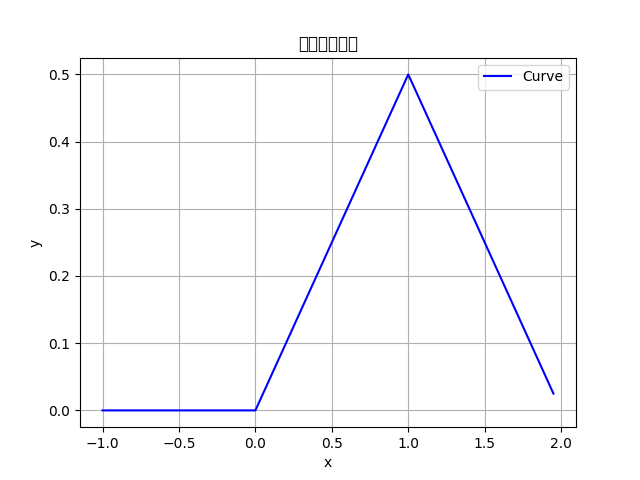
\includegraphics[width=\linewidth]{../figure/n1_3.png} 
        \caption{3-degree \([t_0,t_2]\)}
        \label{fig:image3}
    \end{minipage}
    \caption{\(n=1\)}
    \label{fig:comparison}
\end{figure}

\begin{figure}[h]
    \centering
    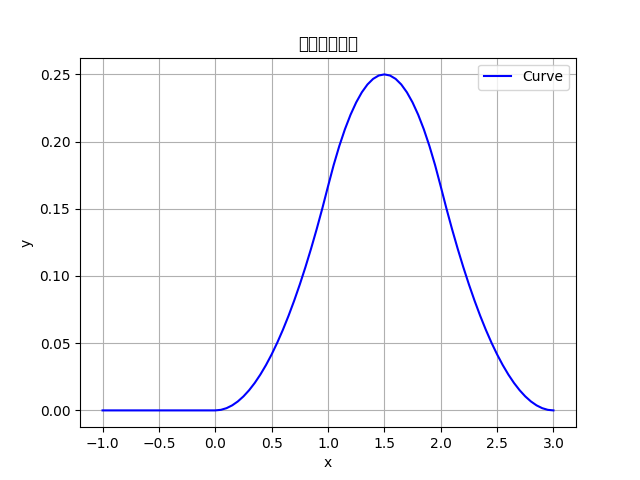
\includegraphics[width=0.6\linewidth]{../figure/n2.png}
    \caption{\(n=2\)}
\end{figure}

To best present the step-like difference table, please note that the order in which the images are generated does not correspond to the actual difference sequence. It is recommended to view the images in the following order for proper correspondence:
\[
\begin{array}{cccc}
     TruncatedPower\_2\_0\_0  \\
     TruncatedPower\_2\_1\_1&TruncatedPower\_2\_0\_1\\
TruncatedPower\_2\_2\_2&TruncatedPower\_2\_1\_2&TruncatedPower\_2\_0\_2\\
TruncatedPower\_2\_3\_3&TruncatedPower\_2\_2\_3&TruncatedPower\_2\_1\_3&TruncatedPower\_2\_0\_3
\end{array}
\]

\section*{G. Sphere curve fitting}

To fit a spherical curve, a stereographic projection coordinate transformation is applied. The curve is mapped onto a plane, fitted, and then inverse-mapped back into 3D space. As shown in the figure, the fitted curve almost completely overlaps with the original curve.
\begin{figure}[h]
    \centering
    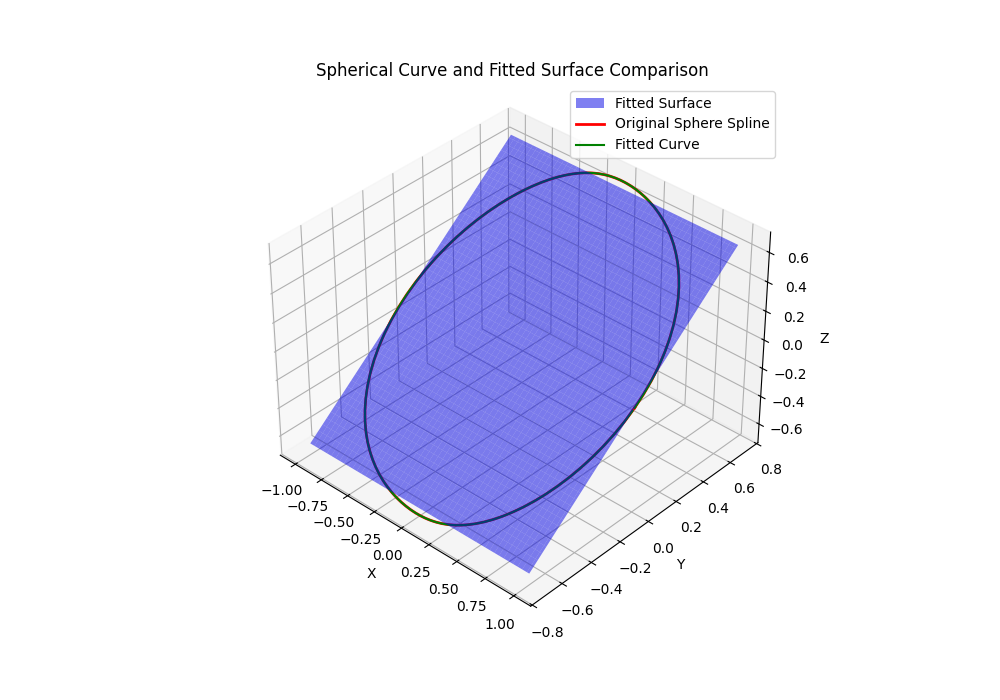
\includegraphics[width=0.6\linewidth]{../figure/Sphere.png}
    \caption{Sphere curve}
\end{figure}

% ===============================================
\subsection*{ \center{\normalsize {Acknowledgement}} }
\printbibliography

\end{document}